\section{Polarization Cameras in the Maritime Domain}
Light behaves as a transverse wave, with its electromagnetic field oscillating in a plane perpendicular to the direction in which it travels.
Similar to how color filters are used to separate different oscillation frequencies, i.e. colors, of light, polarization filters can be used to separate different oscillation directions, i.e. polarizations, of light.
This gives us a new set of tools to analyze the scene, which is be particularly useful in the maritime domain where the water surface is a reflective surface with a distinct polarization signature.

\subsection{Polarization Properties of Reflected Light}
When light is reflected off a surface, its polarization state changes \cite[34]{lingUniversityPhysicsVolume2016}.
This is illustrated in Figure \ref{fig:polarized_reflection} where the unpolarized light reflected off a surface becomes partially polarized.
\begin{figure}[H]
    \centering
    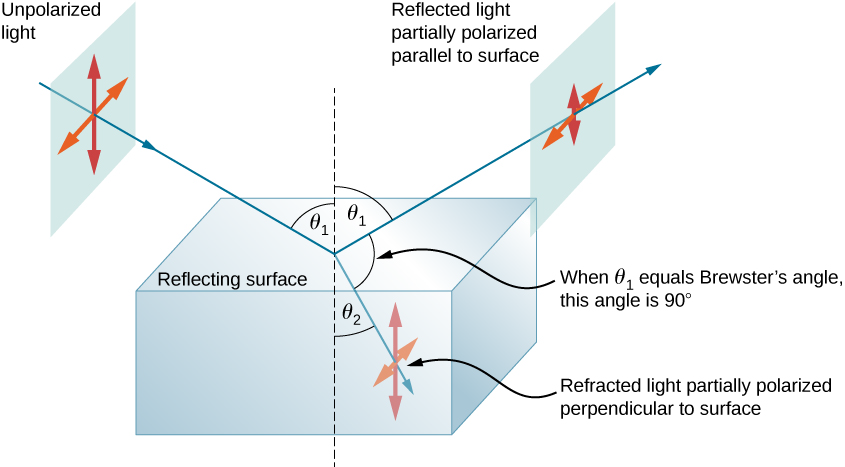
\includegraphics[width=.8\linewidth]{figures/polarization/reflaction.png}
    \caption{Polarization by reflection.
        \cite[Figure 1.38]{lingUniversityPhysicsVolume2016}}
    \label{fig:polarized_reflection}
\end{figure}


Unpolarized light can be described as a sum of two orthogonal linear polarizations $R_\perp$ and $R_\parallel$, where $R_\perp$ is perpendicular to the plane of incidence and $R_\parallel$ is parallel to the plane of incidence  \cite{FresnelEquations2024}.
These two components are referred to as s-polarized and p-polarized light, respectively.
Their reflection coefficients differ and are given by the Fresnel equations below \cite{FresnelEquations2024}:

\begin{align}
    R_\perp =         & \left|{\frac {n_{1}\cos \theta _1-n_{2}\cos \theta _2}{n_{1}\cos \theta _1+n_{2}\cos \theta _2}}\right|^{2}
                      & 
    R_\parallel     = & \left|{\frac {n_{1}\cos \theta _2-n_{2}\cos \theta _1}{n_{1}\cos \theta _2+n_{2}\cos \theta _1}}\right|^{2}
\end{align}

Where  $\eta_1$ and $\eta_2$ are the refractive indices of the two media,
$\theta_i$ is the angle of incidence and $\theta_r$ is the angle of refraction.
Using the trigonometric identity $ \cos^2{\left(\theta_2 \right)} = 1- \sin^2{\left(\theta_2 \right)}$ and Snell's law $\eta_1 \sin{\left(\theta_1 \right)} = \eta_2 \sin{\left(\theta_2 \right)}$ the angle of refraction, $\theta_2$ can be removed, and the equations can be rewritten as:

\begin{align}
    R_\perp =         & \left|{\frac {n_{1}\cos \theta _1-n_{2}{\sqrt {1-\left({\frac {n_{1}}{n_{2}}}\sin \theta _1\right)^{2}}}}{n_{1}\cos \theta _1+n_{2}{\sqrt {1-\left({\frac {n_{1}}{n_{2}}}\sin \theta _1\right)^{2}}}}}\right|^{2}
                      & 
    R_\parallel     = & \left|{\frac {n_{1}{\sqrt {1-\left({\frac {n_{1}}{n_{2}}}\sin \theta _1\right)^{2}}}-n_{2}\cos \theta _1}{n_{1}{\sqrt {1-\left({\frac {n_{1}}{n_{2}}}\sin \theta _1\right)^{2}}}+n_{2}\cos \theta _1}}\right|^{2}
\end{align}


Inserting the refractive index of air, $n_1 = 1$, and the refractive index of water, $n_2 = 1.33$, the reflectance can be calculated and plotted as a function of the angle of incidence, $\theta_1$, alone as shown in Figure \ref{fig:brewster0}.
The \gls{dolp} is the degree to which light is polarized and can be defined as the ratio between the difference and the sum of the two polarizations components.
The \gls{dolp} is plotted in Figure \ref{fig:brewster1}.
At one particular angle of incidence, $\theta_B$, known as the Brewser angle, $R_\parallel$ becomes zero, and the reflected light is completely s-polarized \cite{BrewsterAngle2024}:
\begin{align}
    \theta_B & = \arctan{\frac{n_2}{n_1}} & DoLP= & \frac{\left | R_\perp - R_\parallel \right |}{R_\perp + R_\parallel}
\end{align}

\begin{figure}[H]
    \centering
    \begin{subfigure}{.5\textwidth}
        \centering
        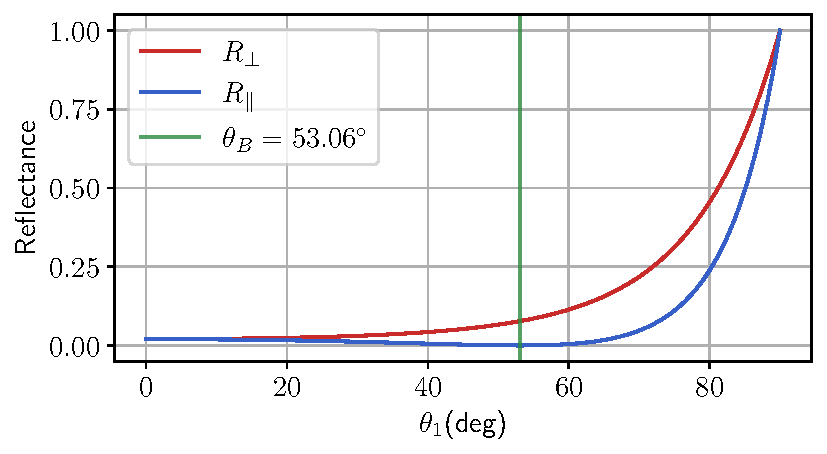
\includegraphics[width=\textwidth]{figures/pol_plots/brewster0.pdf}
        \caption{Reflectance of S and P polarized light of water.}
        \label{fig:brewster0}
    \end{subfigure}%
    \begin{subfigure}{.5\textwidth}
        \centering
        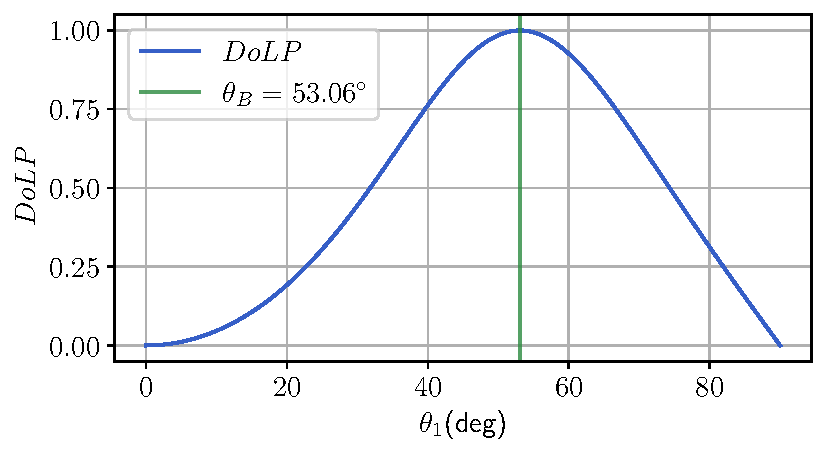
\includegraphics[width=\textwidth]{figures/pol_plots/brewster1.pdf}
        \caption{\gls{dolp} of light reflected off water.}
        \label{fig:brewster1}
    \end{subfigure}
    \caption{Reflectance and \gls{dolp} of light reflected off water as a funcion of of the angle of incidence.
        The Brewster angle is marked with a vertical line.}
    \label{fig:test}
\end{figure}




\subsection{Estimating Polarization Properties of Light using Polarizers}
In polarized light, the electromagnetic oscillations trace an elliptical path, which simplifies to a circular or straight line for pure circular or linear polarization, respectively.
When light passes through a linear polarizer, the electric field is filtered, allowing only the component aligned with the polarizer to continue through.
By aligning four linear polarizers at 45-degree intervals, the \glsfirst{dolp} and \glsfirst{aolp} can be determined as shown in Figure \ref{fig:polarization_calculation}.

\begin{figure}[H]
    
    \begin{minipage}{.48\textwidth}
        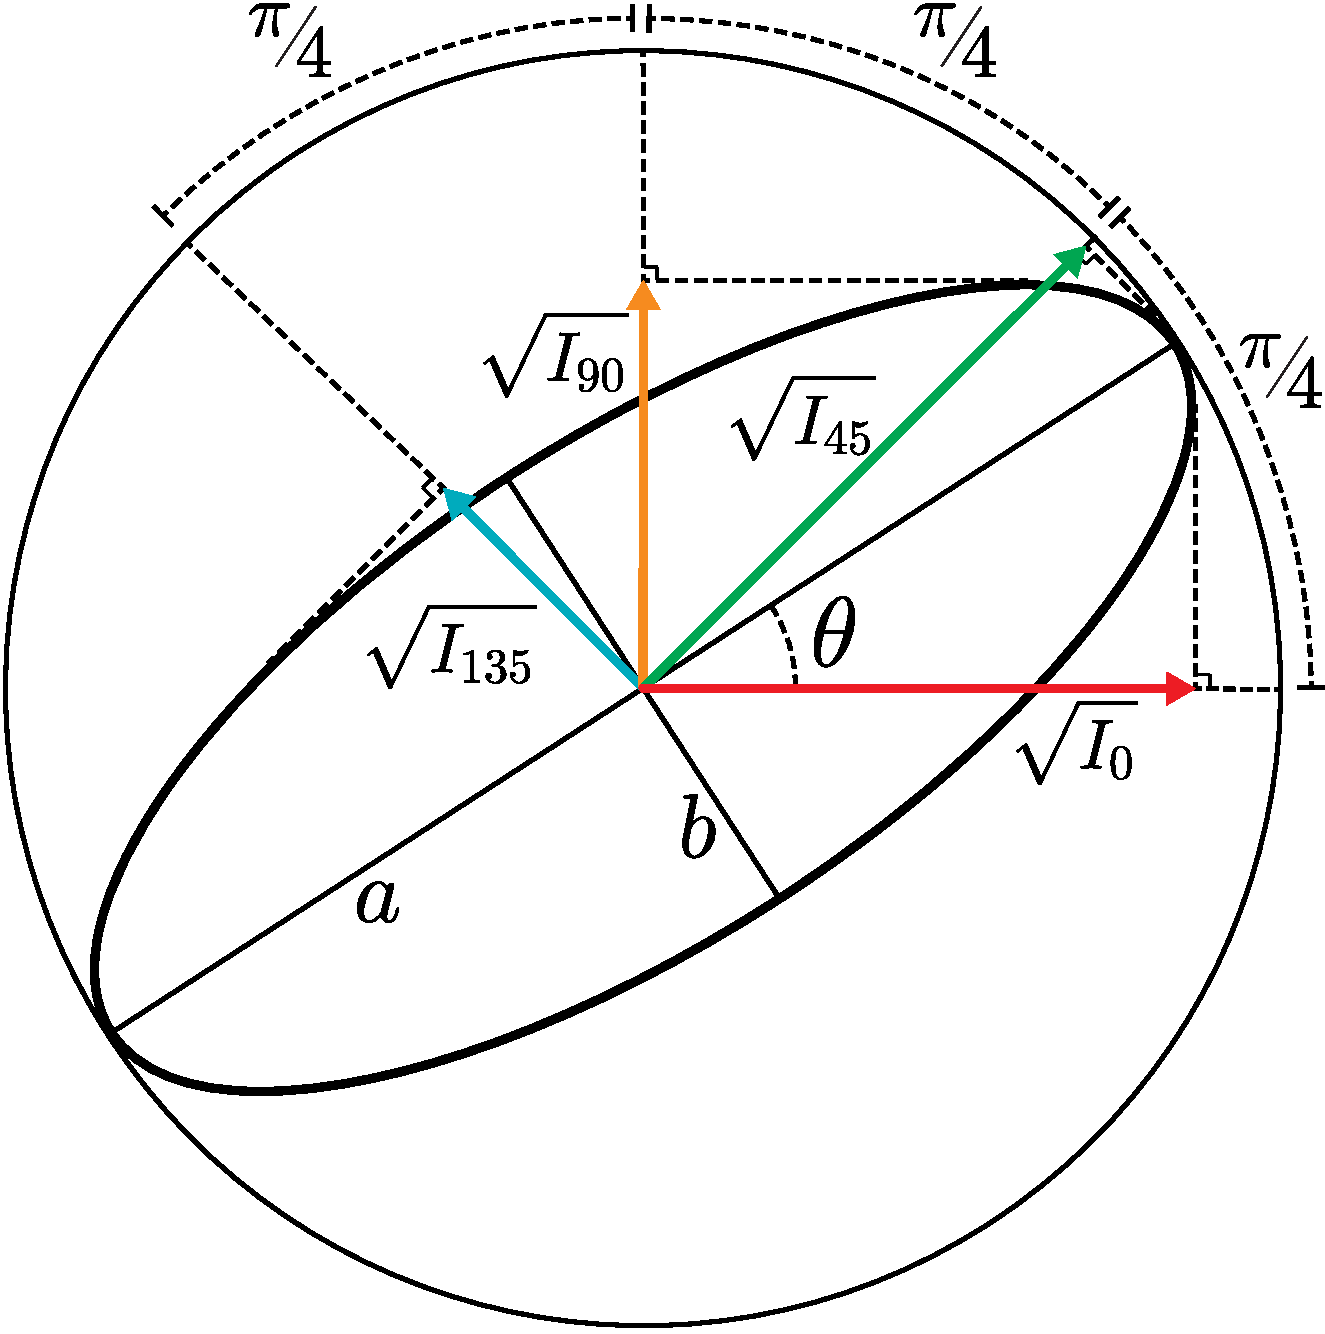
\includegraphics[width=\textwidth]{figures/polarization_sketch.pdf}
    \end{minipage}
    \hfill
    \begin{minipage}{.48\textwidth}
        \begin{alignat}{3}
             & \mathrlap{\cos\theta \cdot a\cos t -  \sin\theta \cdot b\sin t}                & 
             &                                                                                & 
             &                                                                                   \\
             &                                                                                & 
             & = \mathrlap{\sqrt{a^2\cos^2\theta+b^2\sin^2\theta} \cos(\omega + \phi)}        & 
             &                                                                                   \\[1em]
             & I_0                                                                            & 
             & = \mathrlap{a^2\cos^2\theta + b^2\sin^2\theta                                } & 
             &                                                                                   \\
             & I_{45}                                                                         & 
             & = \mathrlap{a^2\cos^2(\theta-\frac{\pi}{4}) + b^2\sin^2(\theta-\frac{\pi}{4})} & 
             &                                                                                   \\
             & I_{90}                                                                         & 
             & = \mathrlap{a^2\sin^2\theta + b^2\cos^2\theta                                } & 
             &                                                                                   \\
             & I_{135}                                                                        & 
             & = \mathrlap{a^2\sin^2(\theta-\frac{\pi}{4}) + b^2\cos^2(\theta-\frac{\pi}{4})} & 
             &                                                                                   \\[1em]
             & S_0                                                                            & 
             & = I_0 + I_{90}                                                                 & 
             & = a^2+b^2                                                                         \\
             & S_1                                                                            & 
             & = I_0 - I_{90}                                                                 & 
             & =(a^2-b^2)\cos(2x)                                                                \\
             & S_2                                                                            & 
             & = I_{45} - I_{135}                                                             & 
             & =(a^2-b^2)\sin(2x)                                                                \\[1em]
             & DoLP                                                                           & 
             & =\frac{a^2-b^2}{a^2+b^2}                                                       & 
             & = \frac{\sqrt{S_1^2 + S_2^2}}{S_0}                                                \\
             & AoLP                                                                           & 
             & =  \theta                                                                      & 
             & = \frac{1}{2}\arctan{\left(\frac{S_2}{S_1}\right)}
        \end{alignat}
    \end{minipage}%
    
    \caption{How four linear polarizers placed at $45^\circ$ intervals can be used to calculate the \gls{dolp} and \gls{aolp} of polarized light. The intensities  \label{fig:polarization_calculation}}
\end{figure}

\section{Polarization Cameras}
The sensor rig is equipped with two TRI050S1-QC cameras from Lucid Vision Labs.
The cameras are have a 5MP \gls{cpfa} sensor, depicted in Figure \ref{fig:cpfa}, capabale of capturing both color and polarization information.

\begin{figure}[H]
    \begin{subfigure}[B]{.48\textwidth}
        \centering
        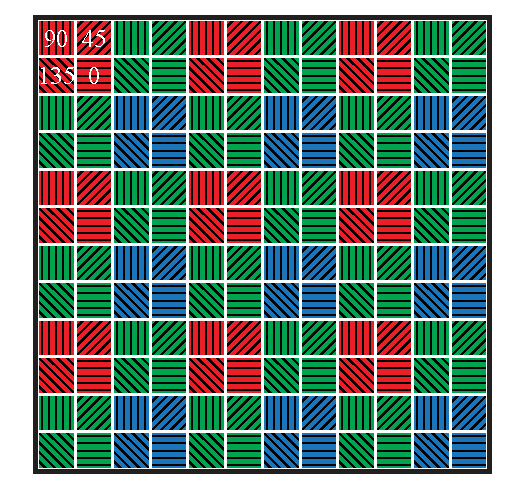
\includegraphics[width=\textwidth]{figures/sensor_layout.pdf}
        \caption{\gls{cpfa}. The numbers represents the filter angles.\label{fig:cpfa}}
    \end{subfigure}
    \hfill
    \begin{subfigure}[B]{.48\textwidth}
        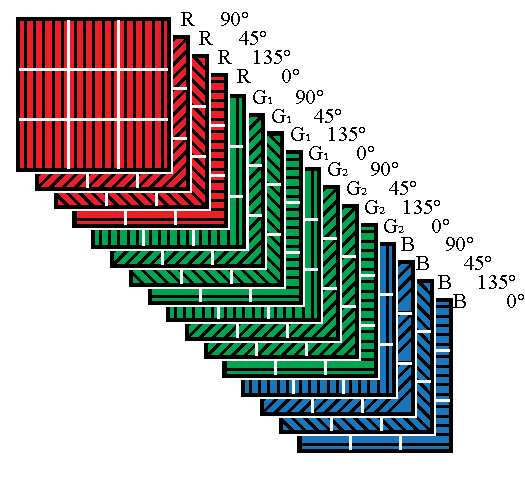
\includegraphics[width=\textwidth]{figures/sensor_packaging.pdf}
        \caption{Reordered view of \ref{fig:cpfa}. \label{fig:cpfa_reorder}}
    \end{subfigure}
    \caption{A 12\times12 slice of the \gls{cpfa} used in TRI050S1-QC cameras \cite{lucidvisionlabsTritonMPPolarized2020}, and how the the data can be reorderd as a 3\times3 image with 16 channels. \label{fig:polarization_sensor}}
\end{figure}

\subsection{A Simple Color-Polarization Demosaicking Approach}
Similar to how color demosacking is used to estimate the missing color channels from a Bayer filter array sensor, color-polarization demosaicking is needed to estimate the missing polarization channels from a \gls{cpfa} sensor.
Several methods already exists for performing accurate color-polarization demosaicking \cite{morimatsuMonochromeColorPolarization2020}\cite{morimatsuMonochromeColorPolarization2021}\cite{nguyenTwoStepColorPolarizationDemosaicking2022a}, but we propose a simple linear method that can be implemented as a single convolutional layer.
The method estimates $S0$, $S1$, and $S2$ for each color channel at every pixel, i.e. it transforms the $n \times m \times 1$ raw \gls{cpfa} image into a $n \times m \times 9$ image.

First the raw \gls{cpfa} input image is permuted into a $(n/4) \times (m/4) \times 16$ image, where the 16 channels correspond to the different color and polarization filters as depicted in Figure \ref{fig:cpfa_reorder}.
This can be done by the following tensor operations:
\begin{figure}[H]
    \centering
    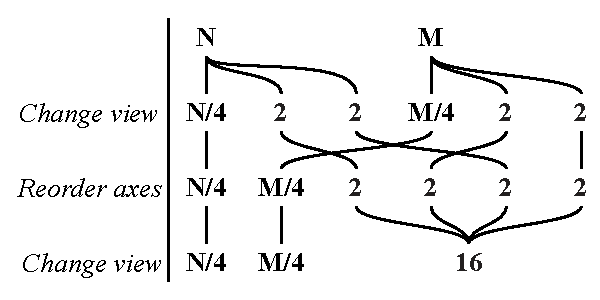
\includegraphics[width=.6\textwidth]{figures/transformation.pdf}
    \caption{Permutations from a $n \times m \times C $ tensor to a $(n/4) \times (m/4) \times (C\times 16)$ tensor. \label{fig:reorder_operations}}
    
\end{figure}%
A custom CUDA kernel was written to unpack raw camera data and perform this permutation in one step, but the same result can be achieved with a series of reshape and transpose operations in PyTorch.
Then a single convolutional layer is applied to obtain a $(n/4)*(m/4)*144$ image.
Finally, the image is permuted back to a $n \times m \times 9$ image by reversing the operations in Figure \ref{fig:reorder_operations}.

Using a kernel size of 5 the convolutional layer has $144\times16\times5\times5=57600$ weights.
Since we only use a single convolution operation, the transformation is linear and we can find the least square solution directly, without the use of gradient descent.
The weights were fitted to the The Tokyo Tech dataset, a 12-channel (3 colors \times 4 angles) color-polarization image dataset with 40 scenes \cite{morimatsuMonochromeColorPolarization2020}\cite{morimatsuMonochromeColorPolarization2021}.
To simulate raw \gls{cpfa} images we slect the channel for each pixel with the same color and polarization angle as the corresponding pixel in the \gls{cpfa} image.

To increase the size of the dataset, we used all 16 possible placements of the virtual \gls{cpfa} on each image, by shifting the images up to 3 pixels in each direction.
We also augmented the dataset by flipping the images horizontally and vertically.
Without acces to the exact testing setup used from more advenced methods, we can not say exactly how well our method performs in comparison, but


\begin{figure}[H]
    \begin{subfigure}[T]{.49\textwidth}
        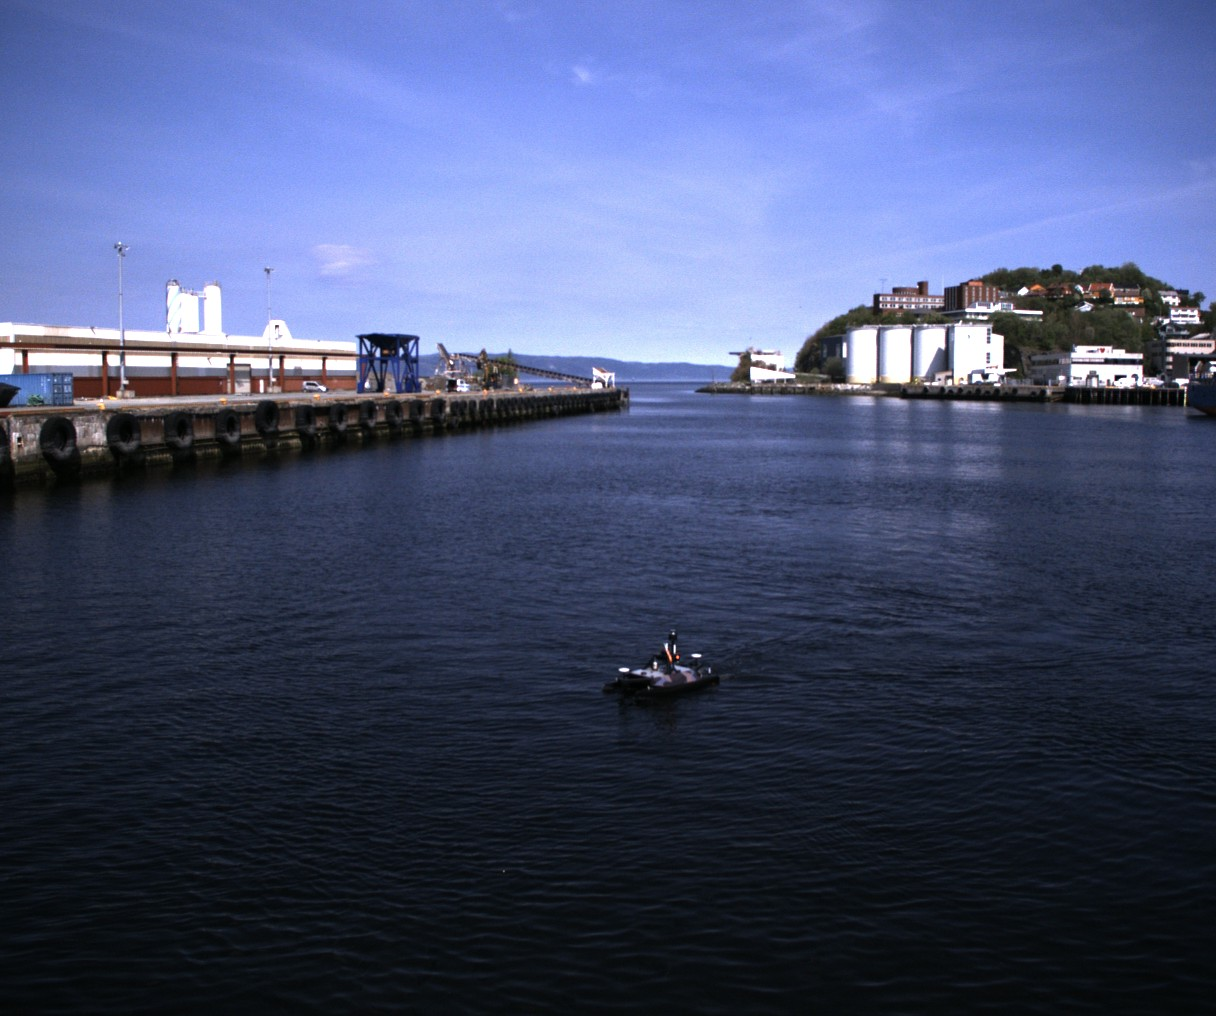
\includegraphics[width=\textwidth]{figures/img_0080_right_s0.jpg}
        \caption{$S_0$, equivalent to what a normal camera would capture.}
    \end{subfigure}
    \hfill
    \begin{subfigure}[T]{.49\textwidth}
        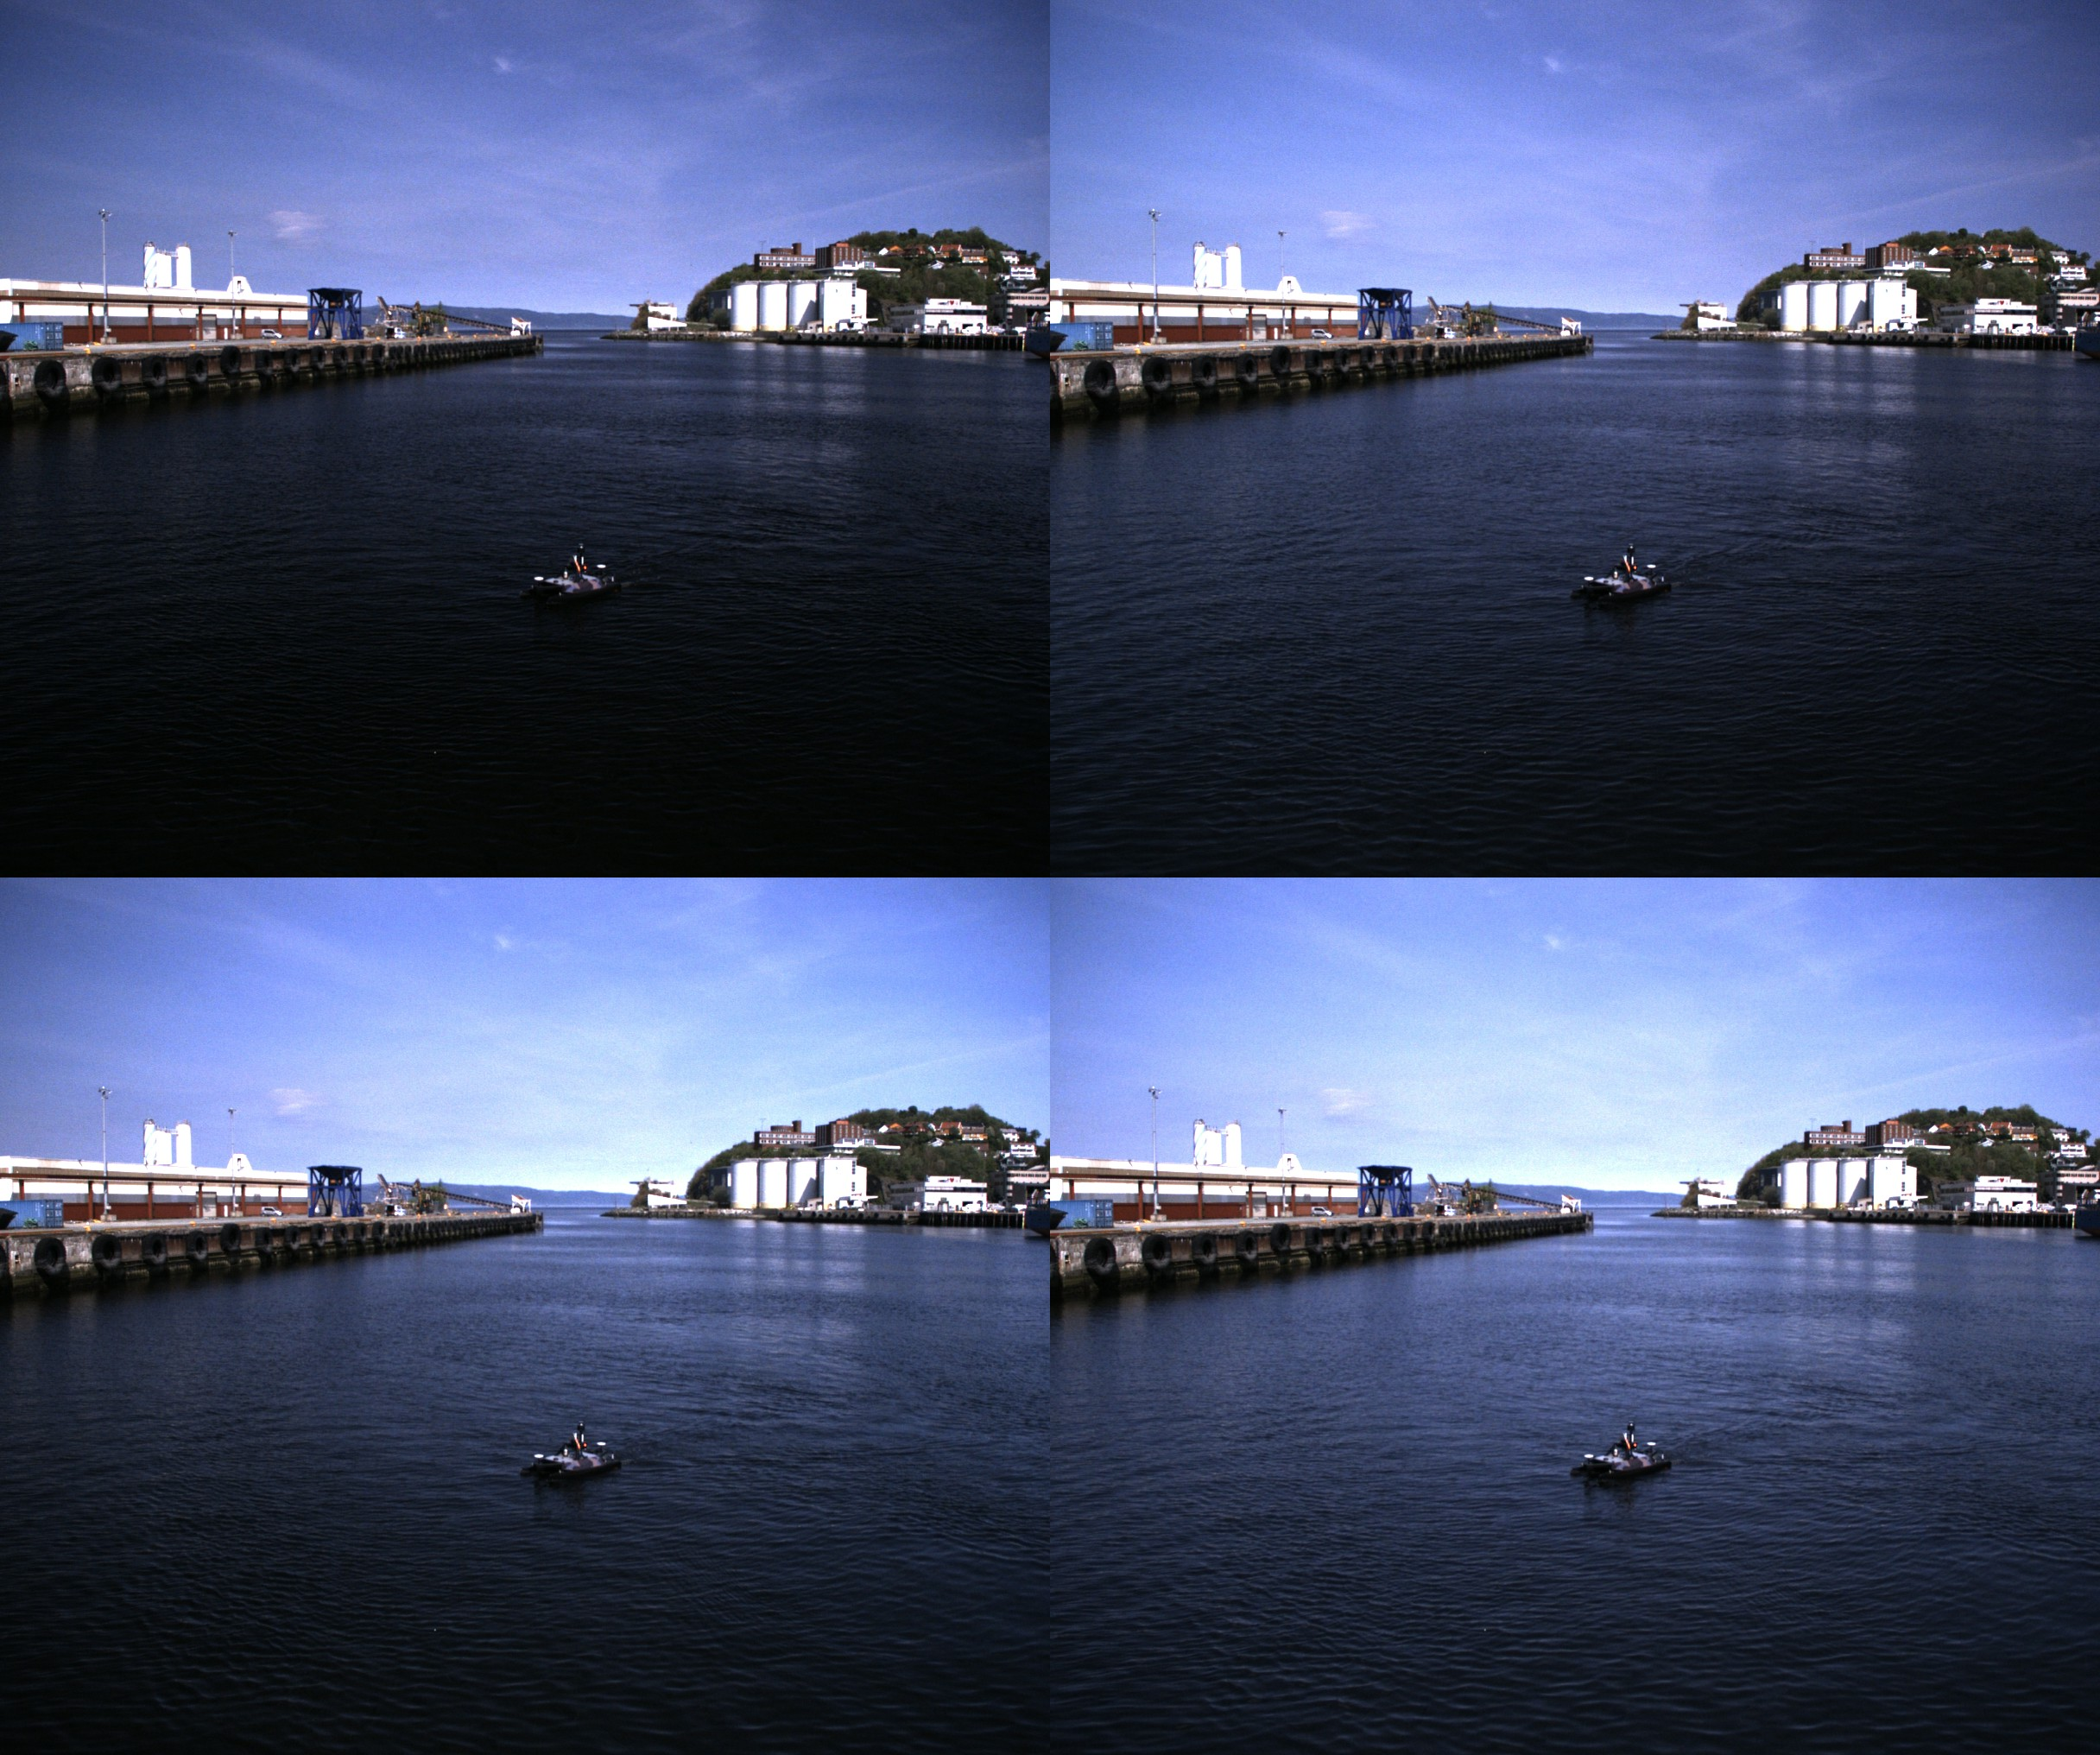
\includegraphics[width=\textwidth]{figures/img_0080_right_inten.jpg}
        \caption{$I90$, $I45$, $I135$, and $I0$.}
    \end{subfigure}
    
    \begin{subfigure}[B]{.49\textwidth}
        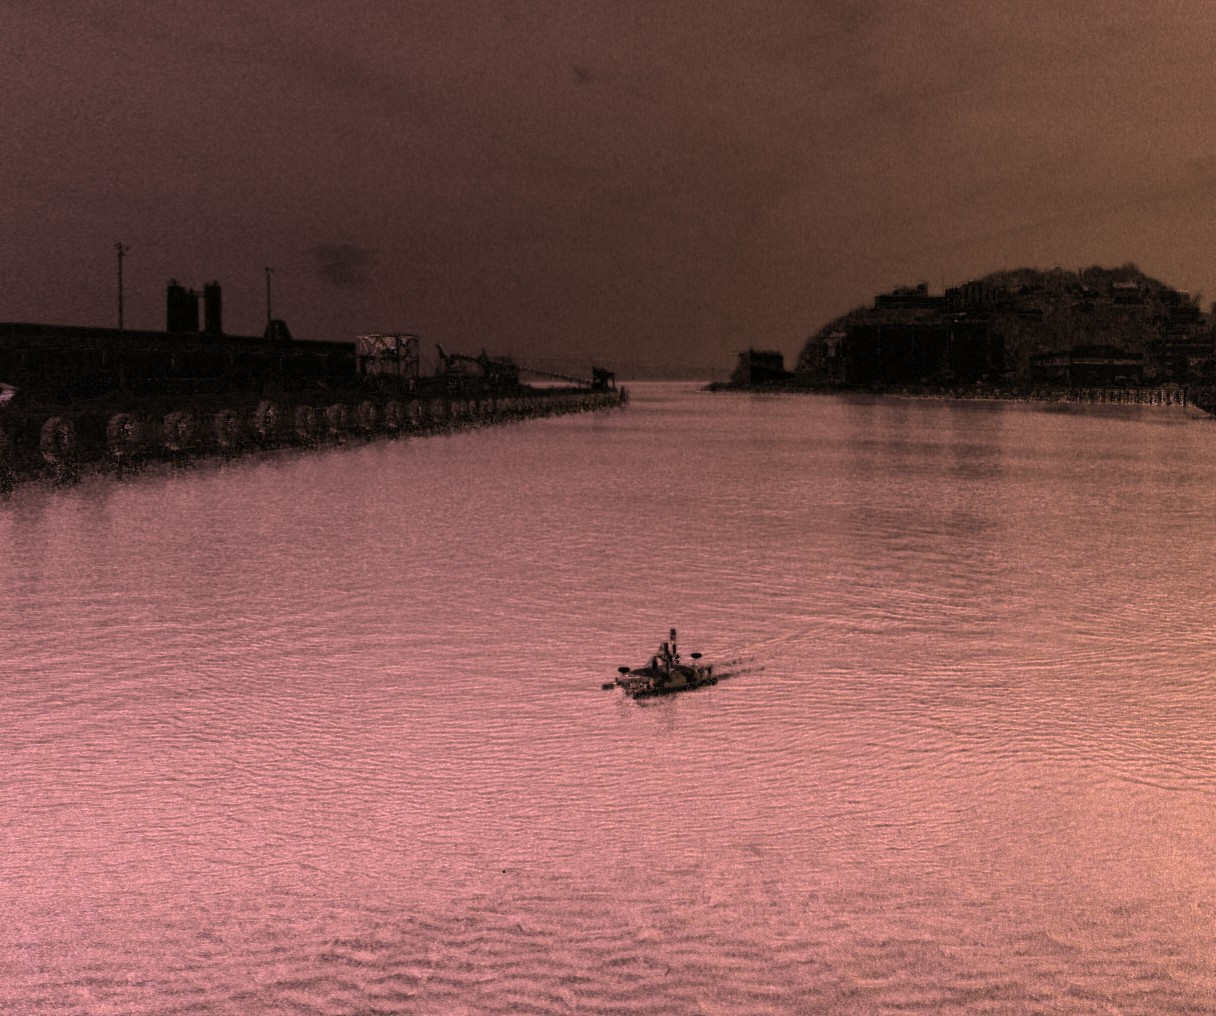
\includegraphics[width=\textwidth]{figures/img_0080_right_pol.jpg}
        \caption{Visualization of \gls{dolp} and \gls{aolp}}
    \end{subfigure}
    \hfill
    \begin{subfigure}[B]{.49\textwidth}
        \centering
        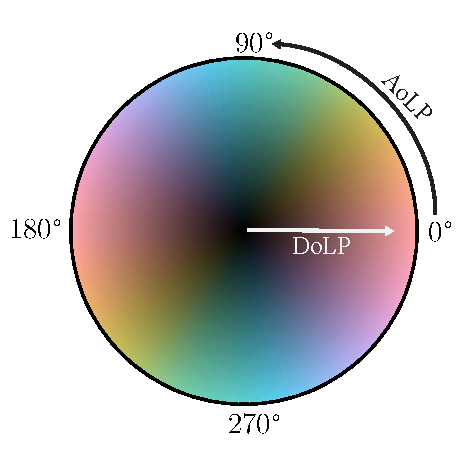
\includegraphics[width=.8\textwidth]{figures/cmap/aolp_dolp_cmap.pdf}
        \vspace{1em}
        \caption{Colormap}
    \end{subfigure}
    \caption{Visualization of an image captured with a color polarization filter array sensor. Note how the polarization information facilitates detection of the small vessel.}
\end{figure}




% \hfill



% \section{Debayering of Color Polarization Images}

% \begin{align*}
%     \text{BT709} = \begin{bmatrix}
%                        0.2126  & 0.7152  & 0.0722  \\
%                        -0.1146 & -0.3854 & 0.5     \\
%                        0.5     & -0.4542 & -0.0458
%                    \end{bmatrix}
% \end{align*}


